% =============================================================================
%  Presentation: "Ignition Heatmaps from SEVIRI FRP" — supervisor meeting
%  Figures: figures/ (existing) and figures/presentation/ (src/plot_presentation_figures.py)
%
%  Compile from docs/presentation/:  latexmk -pdf supervisor_meeting.tex
% =============================================================================
\documentclass[10pt,aspectratio=169]{beamer}

% ------------------------------ Packages -------------------------------------
\usepackage[utf8]{inputenc}
\usepackage[T1]{fontenc}
\usepackage{lmodern}
\usepackage{booktabs}
\usepackage{array}
\usepackage{xcolor}
\usepackage{graphicx}
\usepackage{appendixnumberbeamer}
\graphicspath{{../../figures/}}

% ------------------------------ Custom colors --------------------------------
\definecolor{accent}{RGB}{35, 90, 130}
\definecolor{soft}{RGB}{230, 238, 247}
\definecolor{ember}{RGB}{200, 80, 30}

% ------------------------------ Theme ----------------------------------------
\usetheme[progressbar=frametitle, numbering=fraction, block=fill]{metropolis}
\setbeamertemplate{navigation symbols}{}
\setbeamercolor{progress bar}{fg=accent}
\setbeamercolor{frametitle}{bg=accent}
\setbeamercolor{title separator}{fg=accent}
\setbeamercolor{alerted text}{fg=ember}
\setbeamertemplate{page number in foot}[totalframenumber]

\newcommand{\src}[1]{{\tiny\color{gray}#1}}

% ------------------------------ Title page -----------------------------------
\title{Ignition Heatmaps from SEVIRI Fire Radiative Power}
\subtitle{Master thesis --- progress update and open points}
\author{Rafael Gufler}
\date{October 2026}

% =============================================================================
\begin{document}
% =============================================================================

\begin{frame}[plain]
  \titlepage
\end{frame}

% ---------------------------------------------------------------- Summary ----
\begin{frame}{In one slide}
  \begin{block}{Task}
    Input: 24\,h of SEVIRI FRP hotspots (15-min scans, $\approx 3 \times 4.5$\,km pixels), Portugal 2004--2019.\\
    Output: an \textbf{ignition probability map} --- where did fires $\geq 50$\,ha start in the middle 12\,h?\\
    Ground truth: ICNF fire register (ignition point, start time, burned area).
  \end{block}
  \begin{columns}[T]
    \column{0.5\textwidth}
    \begin{exampleblock}{Where it stands}
      \begin{itemize}
        \item Data pipeline, baseline, two models done
        \item Test 2017--19 evaluated \textbf{once}
        \item AP@5\,km \textbf{0.62} vs.\ 0.50 baseline
        \item AP@10\,km \textbf{0.71} vs.\ 0.59 baseline
      \end{itemize}
    \end{exampleblock}
    \column{0.5\textwidth}
    \begin{alertblock}{To discuss today}
      \begin{itemize}
        \item The heatmap framing and evaluation
        \item Data: SEVIRI 2020+, cloud mask, rekindles
        \item Priorities: covariates, Transformer,\\space--time output, explainability
      \end{itemize}
    \end{alertblock}
  \end{columns}
\end{frame}

% =============================================================================
\section{Data}
% =============================================================================

\begin{frame}{The data: what SEVIRI can see}
  \begin{columns}[T]
    \column{0.58\textwidth}
    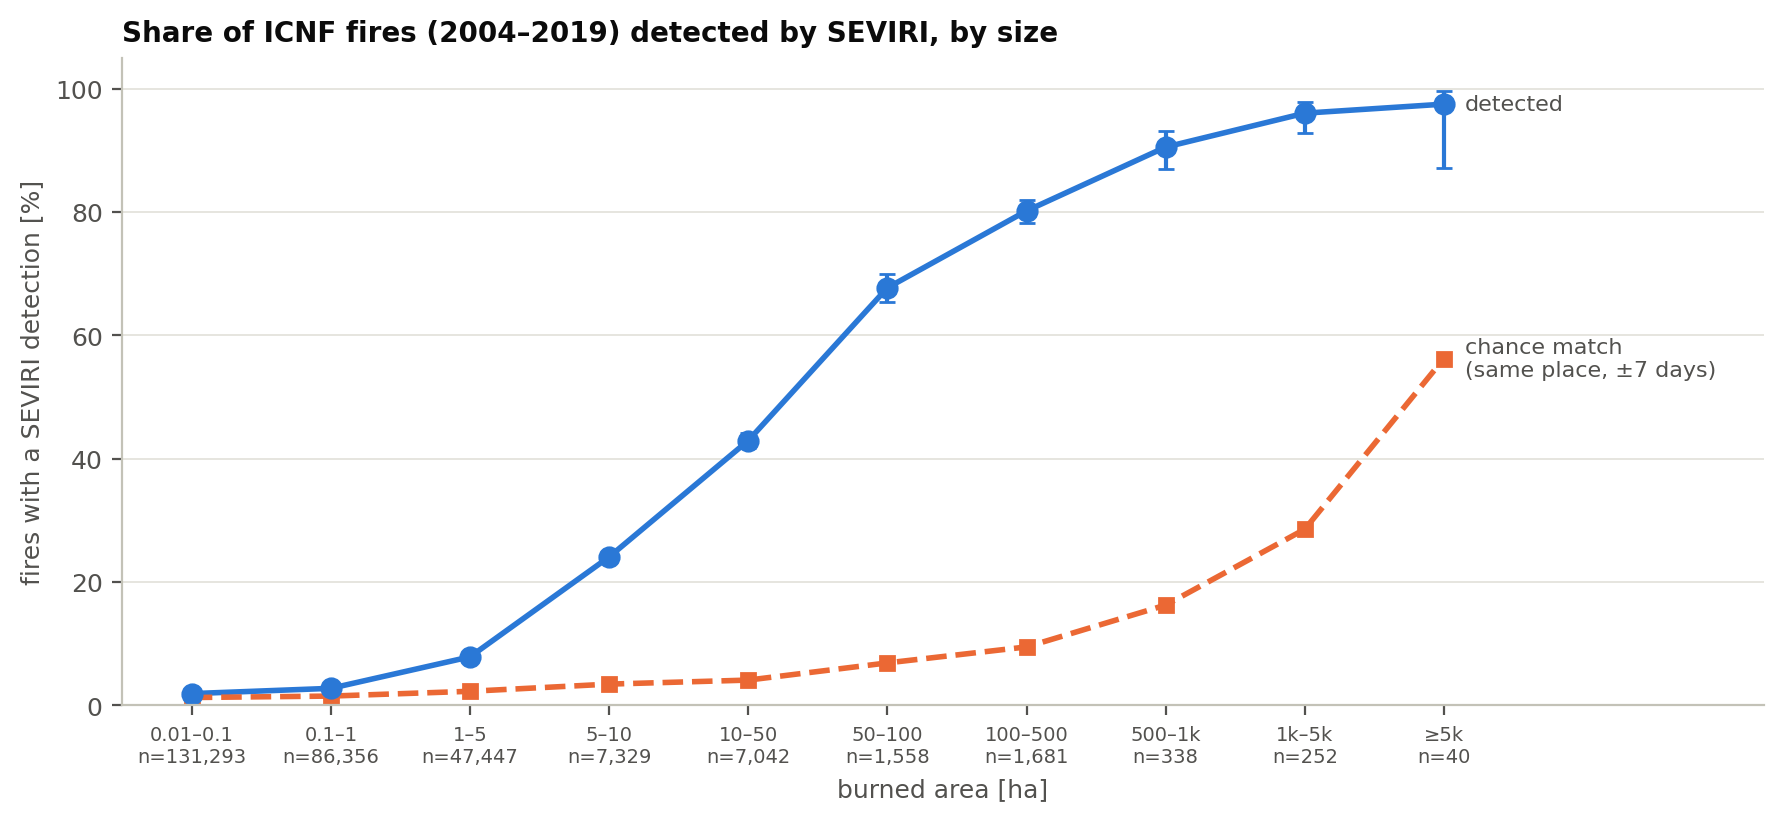
\includegraphics[width=\linewidth]{eda/07_detection_probability.png}
    \column{0.42\textwidth}
    \footnotesize
    \begin{itemize}
      \item \textbf{SEVIRI}: 568k hotspot detections (pixel $\times$ 15-min slot), FRP + confidence; only fire pixels stored
      \item \textbf{ICNF}: 361k fires with coordinates in 2004--2019; only 2,311 $\geq 100$\,ha
      \item Detected: 43\,\% at 10--50\,ha, 68\,\% at 50--100\,ha, $\geq 80$\,\% from 100\,ha
      \item[$\Rightarrow$] \textbf{Targets: fires $\geq 50$\,ha that SEVIRI sees} (2,821)
    \end{itemize}
    \begin{block}{Cleaning findings}
      \footnotesize
      ICNF times are \textbf{local time}, not UTC (lag jumps 0.9\,h at the DST switch).\\
      No confidence filter: it removes the weak, early detections.
    \end{block}
  \end{columns}
\end{frame}

\begin{frame}{Data pipeline}
  \centering
  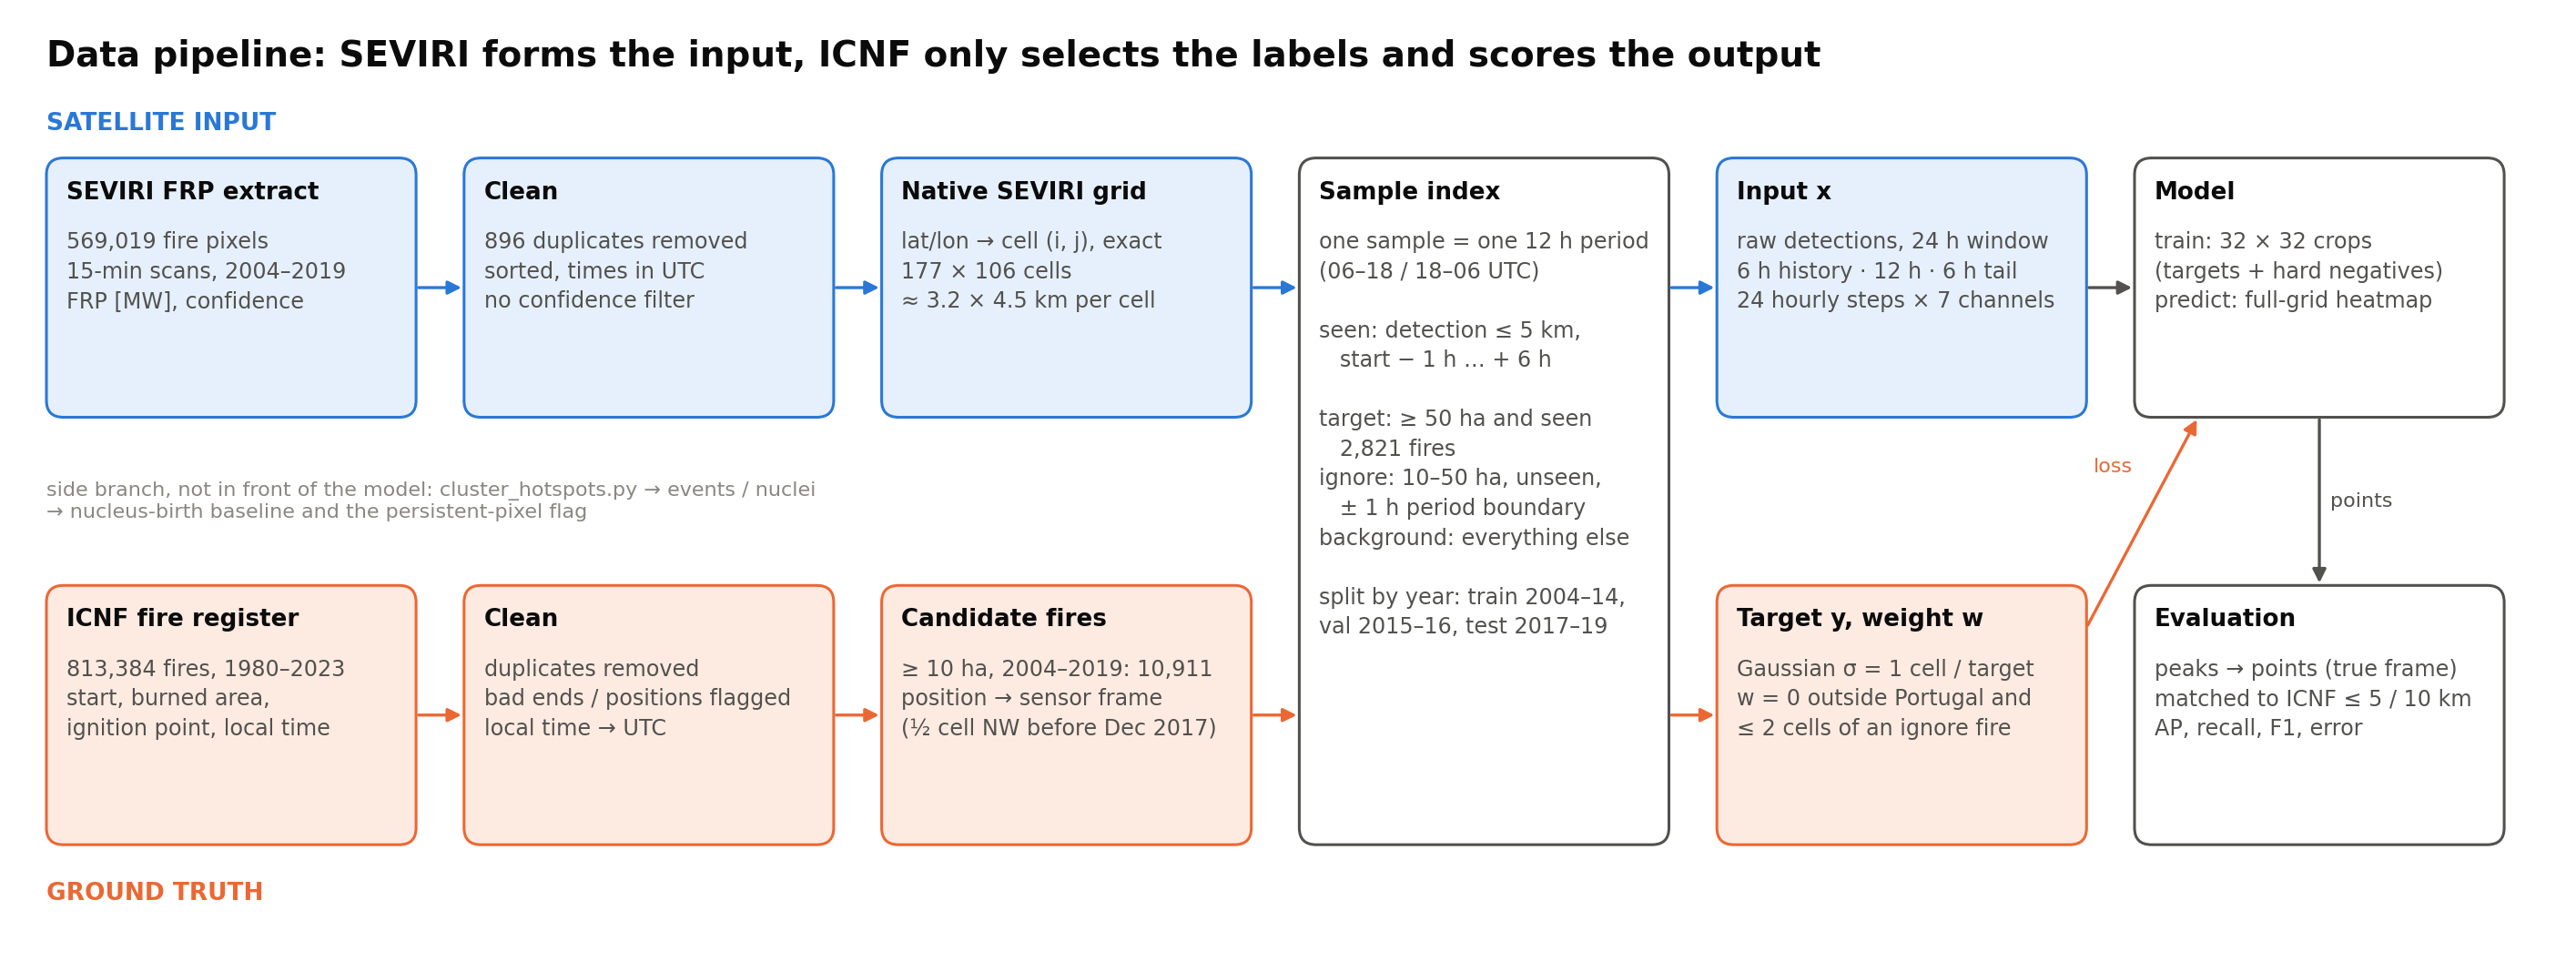
\includegraphics[width=\linewidth]{pipeline/pipeline_overview.png}\\[2pt]
  \small
  Native SEVIRI grid recovered exactly (177 $\times$ 106 cells, no resampling) \quad$\cdot$\quad
  chronological split: train 2004--14 / val 2015--16 / \textbf{test 2017--19 locked}
\end{frame}

\begin{frame}{The core difficulty: simultaneous neighbouring fires}
  \begin{columns}[T]
    \column{0.68\textwidth}
    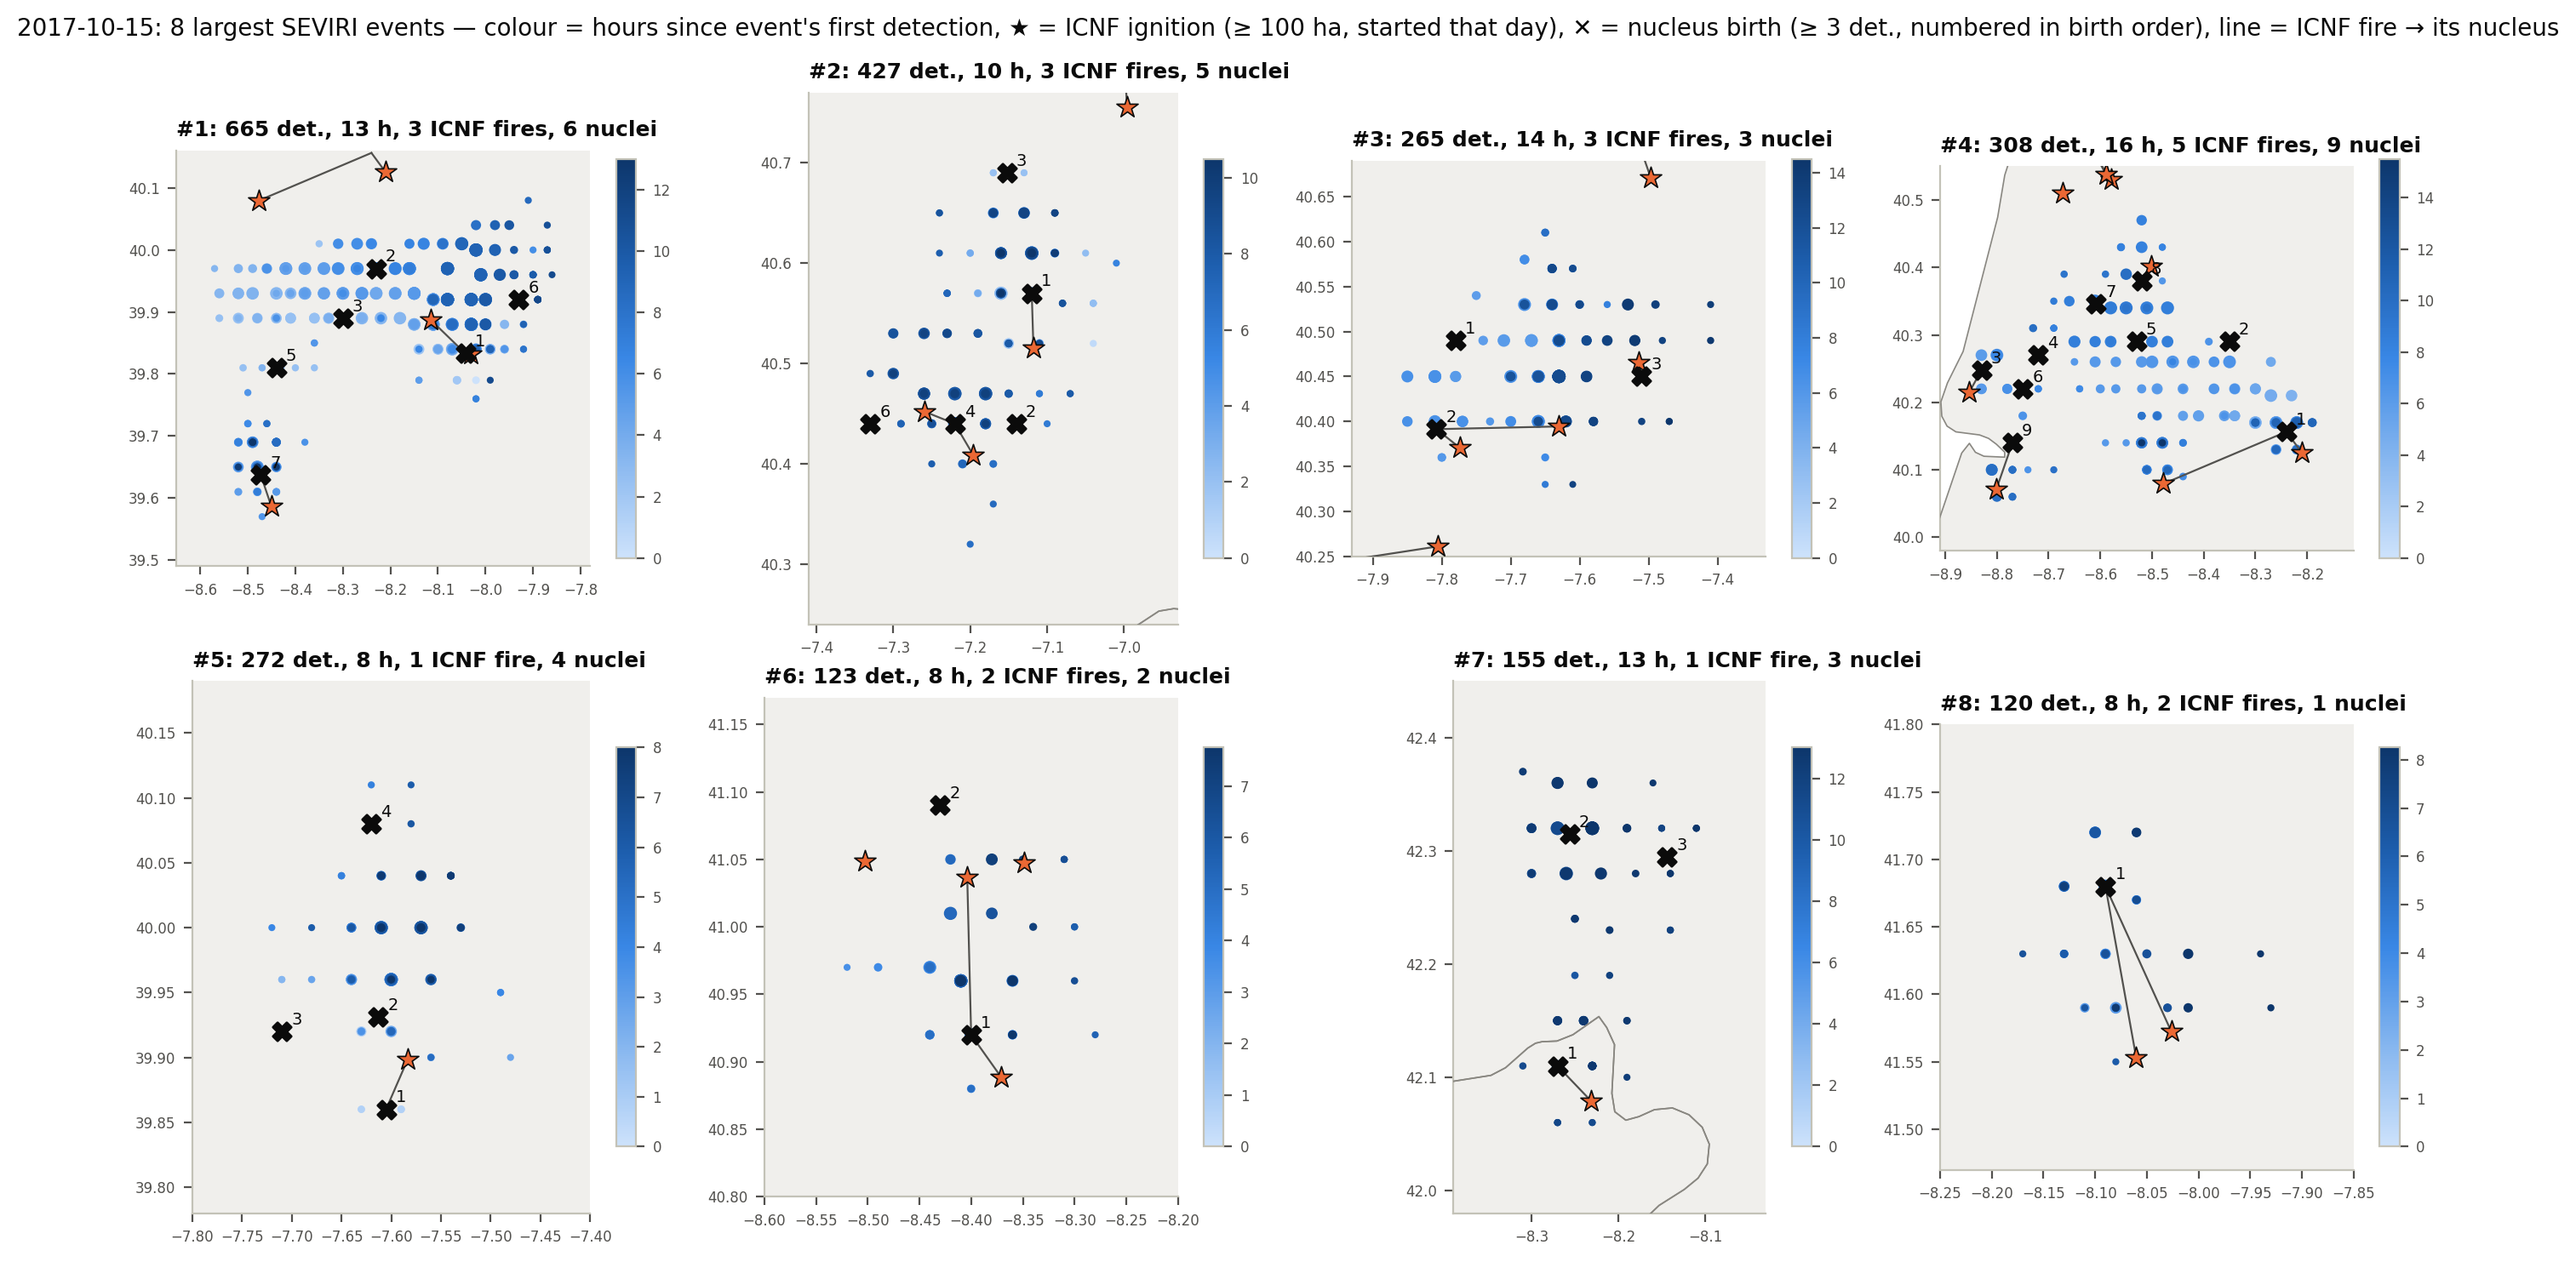
\includegraphics[width=\linewidth]{clustering/events_2017-10-15_panels.png}\\
    \src{2017-10-15: SEVIRI events, ICNF ignitions ($\star$), nucleus births ($\times$)}
    \column{0.32\textwidth}
    \footnotesize
    \begin{itemize}
      \item 1 in 4 large fires has another $\geq 100$\,ha fire within 10\,km on the same day
      \item 1 in 3 shares $> 50$\,\% of its hotspots with another fire
      \item Space--time clustering (6\,km, 6\,h) into events and \textbf{nuclei}: works for isolated fires, fails next to active fires
    \end{itemize}
    \begin{block}{Use of the clustering}
      \footnotesize
      \textbf{Baseline}: every nucleus birth = predicted ignition, ranked by its fire radiative energy.
    \end{block}
  \end{columns}
\end{frame}

% =============================================================================
\section{Approach}
% =============================================================================

\begin{frame}{Framing: ignition heatmaps from raw hotspots}
  \centering
  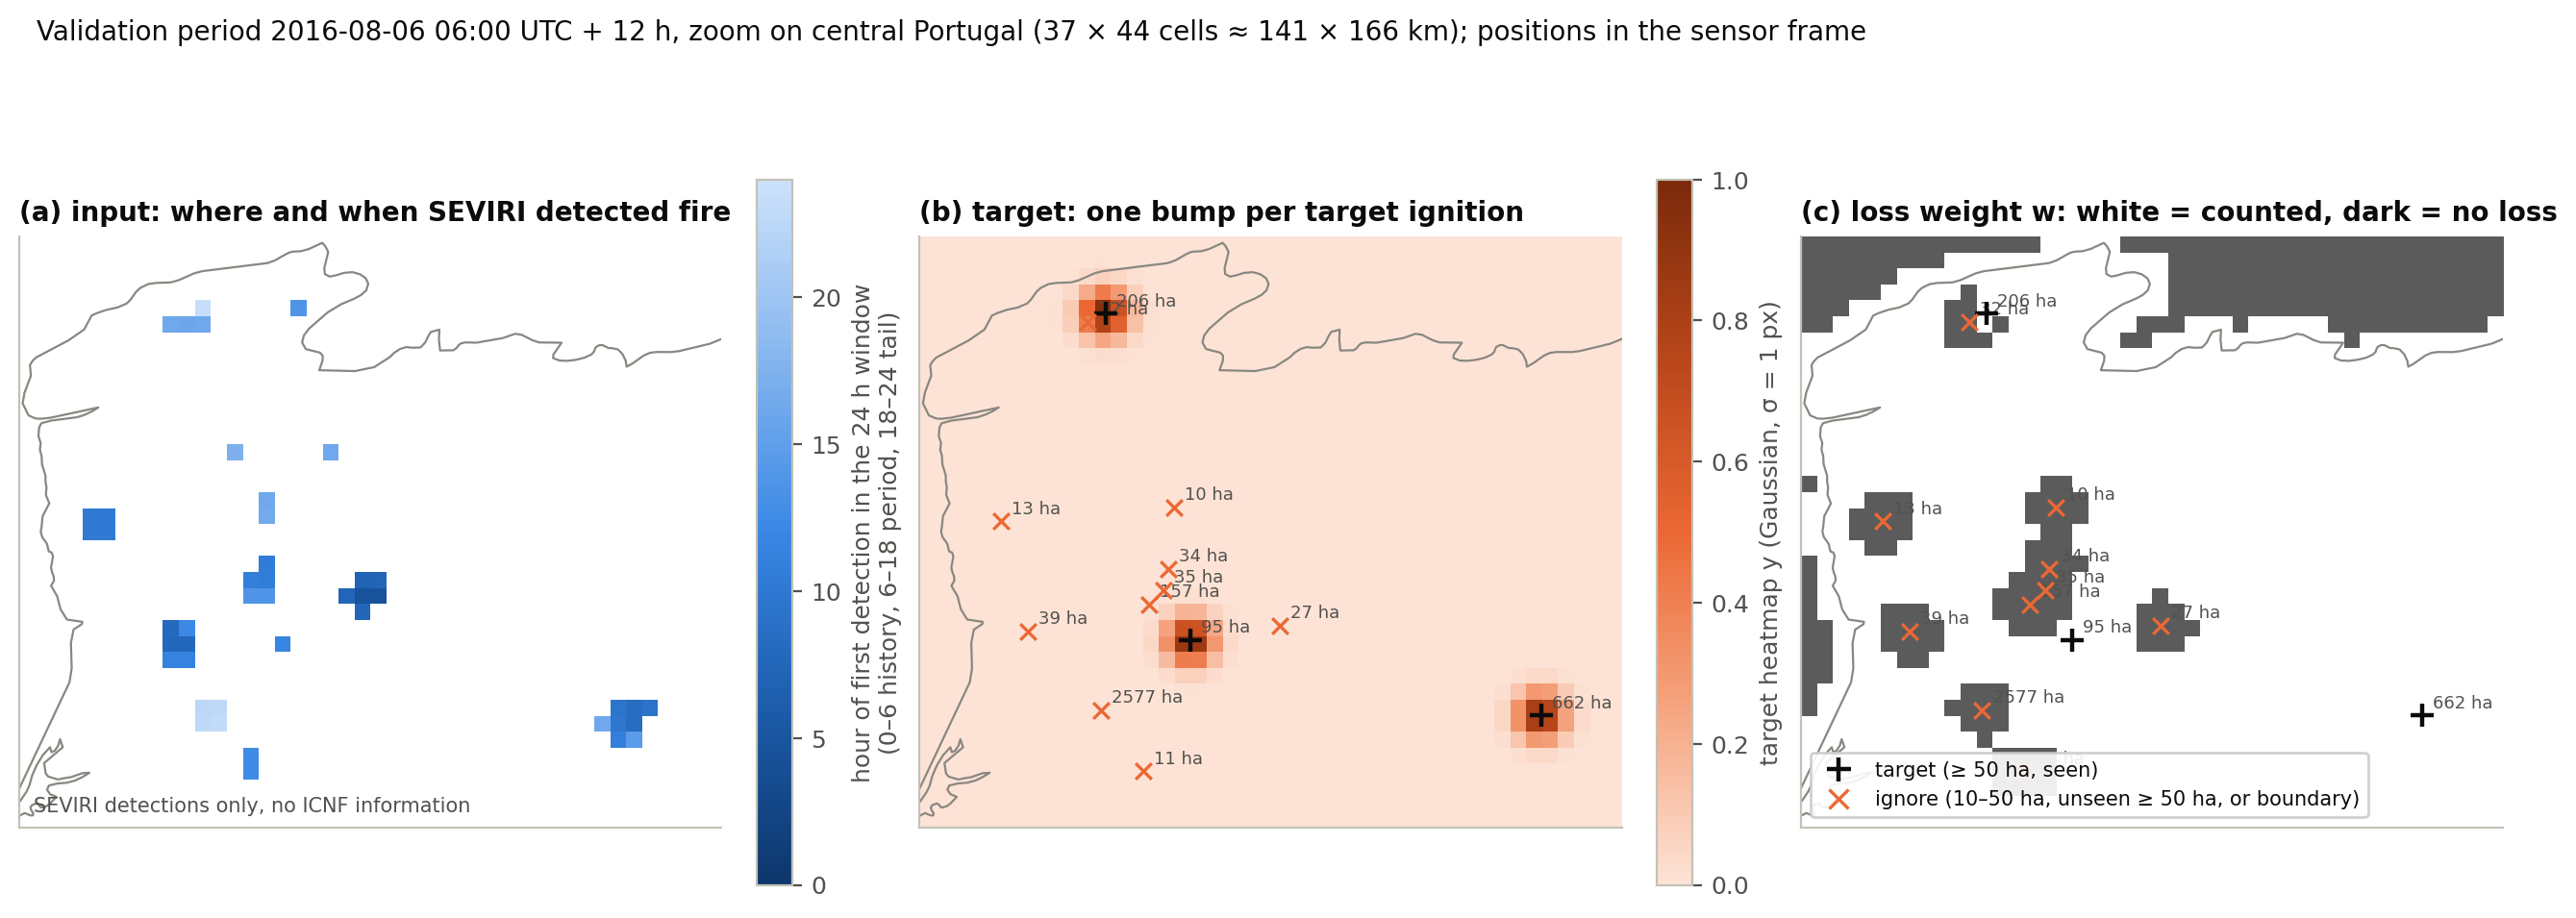
\includegraphics[width=0.88\linewidth]{pipeline/sample_labels.png}
  \small
  \begin{columns}[T]
    \column{0.5\textwidth}
    \begin{itemize}
      \item No hand-made hotspot $\leftrightarrow$ fire assignment: the model learns it
      \item One sample = one 12\,h period; input 6\,h history + 12\,h + 6\,h tail, hourly
    \end{itemize}
    \column{0.5\textwidth}
    \begin{itemize}
      \item Target: Gaussian ($\sigma = 1$ cell) at \emph{every} ignition $\Rightarrow$ 0, 1 or 31 per map
      \item Ignore regions: 10--50\,ha and unseen fires, Spain
    \end{itemize}
  \end{columns}
\end{frame}

\begin{frame}{Model: 3D CNN (main) and ConvLSTM (proposal)}
  \centering
  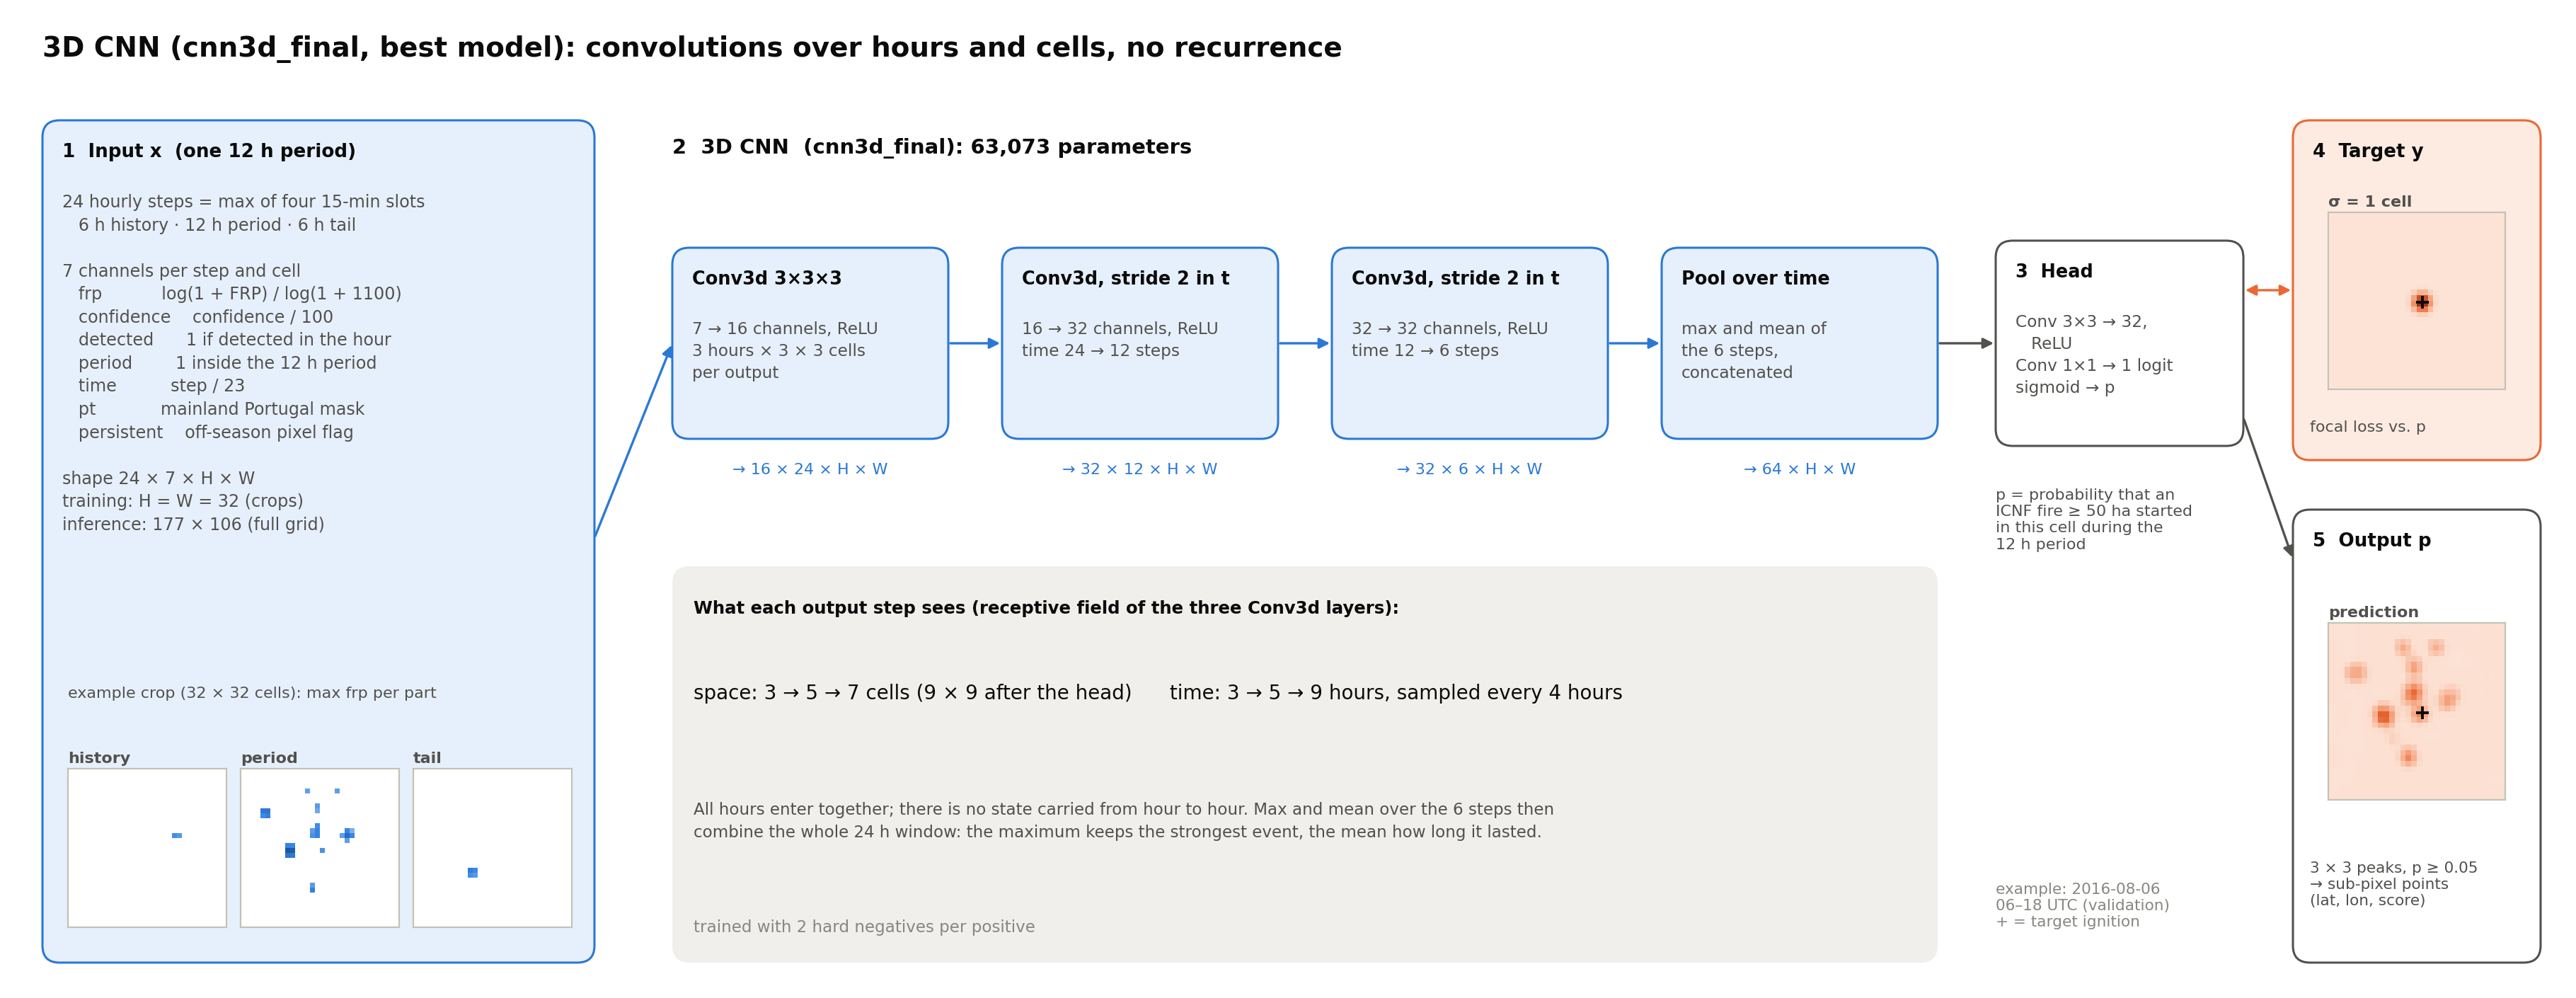
\includegraphics[width=\linewidth]{model/model_cnn3d.png}
  \small
  \begin{columns}[T]
    \column{0.5\textwidth}
    \textbf{Training:} 32 $\times$ 32 crops; one per target + \textbf{2 hard negatives} (fire present, no new ignition); flips; 3 seeds.
    \column{0.5\textwidth}
    \textbf{ConvLSTM:} same input and head, 2 recurrent layers $\times$ 16 channels ($\approx$45k params). Equal on test.
  \end{columns}
\end{frame}

\begin{frame}{Loss and evaluation}
  \begin{columns}[T]
    \column{0.55\textwidth}
    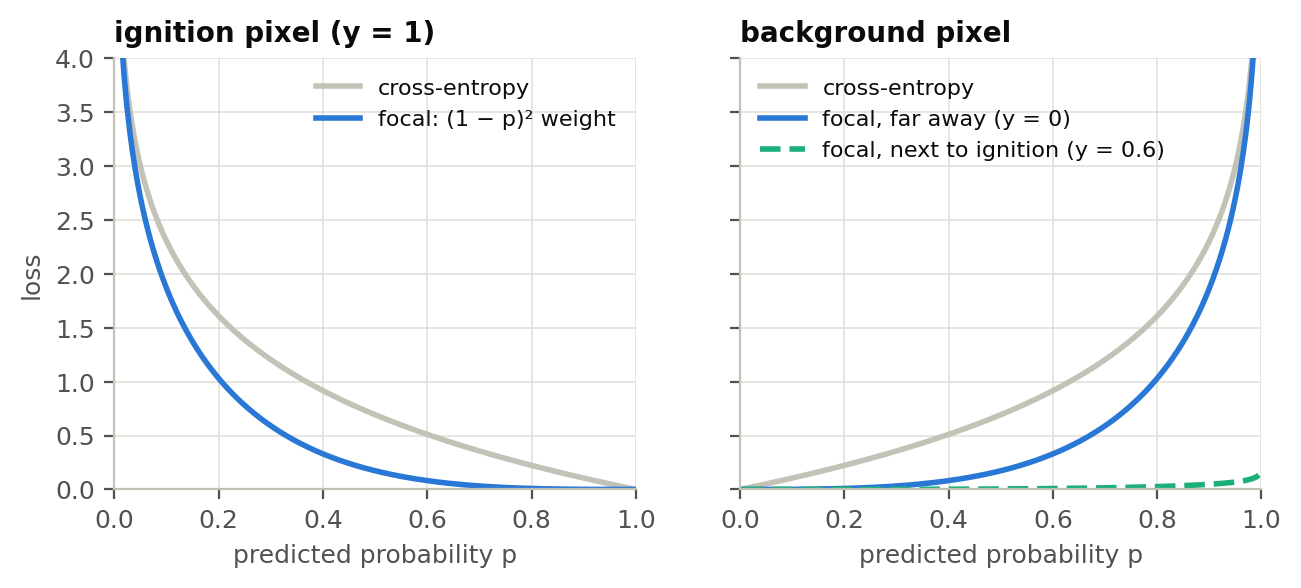
\includegraphics[width=\linewidth]{presentation/focal_loss.png}
    \begin{block}{Focal loss (CornerNet / CenterNet), $\alpha=2,\ \beta=4$}
      \footnotesize
      ignition pixels: $-(1-p)^{\alpha}\log p$\\
      other pixels: $-(1-y)^{\beta}\,p^{\alpha}\log(1-p)$\\[2pt]
      easy pixels down-weighted $\cdot$ near-misses cheap $\cdot$ normalised per ignition
    \end{block}
    \column{0.45\textwidth}
    \small
    \begin{block}{From heatmap to points}
      \footnotesize
      3 $\times$ 3 local maxima, $p \geq 0.05$, sub-pixel centroid $\rightarrow$ lat/lon
    \end{block}
    \begin{block}{Matching and metrics}
      \footnotesize
      Per period, by score: nearest unmatched ICNF ignition within $k$ = hit; near an ignore fire = neither; else false alarm.\\[3pt]
      $k = 5$\,km (location) and $10$\,km (right fire).\\[3pt]
      \textbf{AP} = area under precision--recall: how well scores rank real ignitions, over all thresholds.
    \end{block}
  \end{columns}
\end{frame}

% =============================================================================
\section{Results}
% =============================================================================

\begin{frame}{Finding: a half-pixel geo-referencing offset}
  \begin{columns}[T]
    \column{0.6\textwidth}
    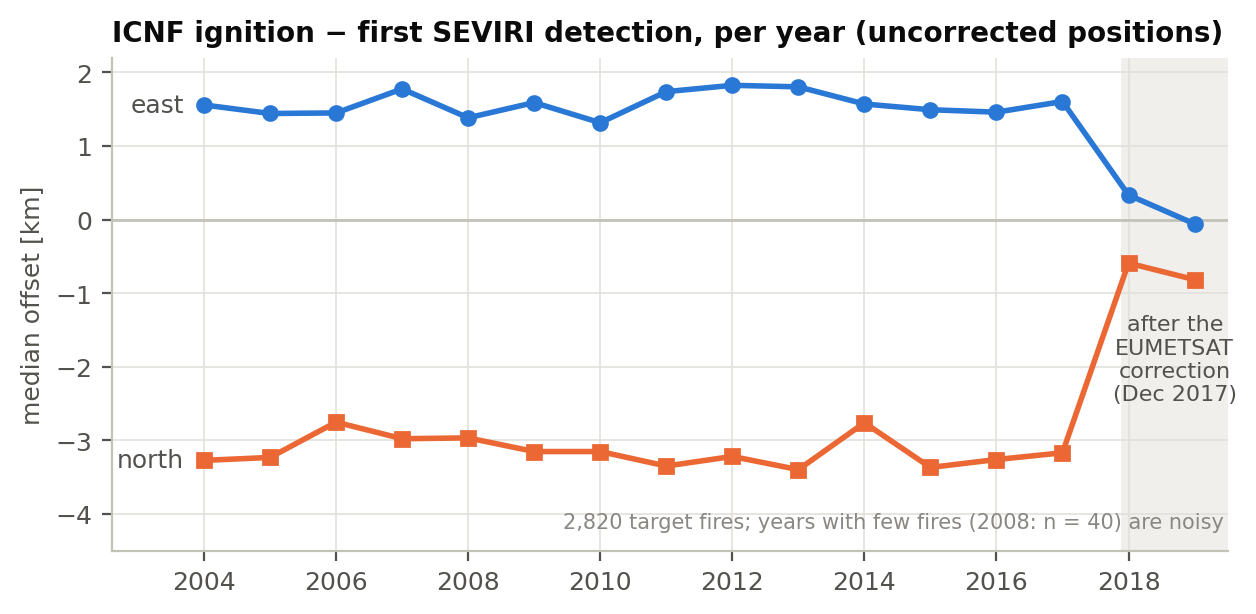
\includegraphics[width=\linewidth]{presentation/georef_offset_by_year.png}
    \column{0.4\textwidth}
    \small
    \begin{itemize}
      \item Symptom: \emph{no flip augmentation} almost doubled AP@5\,km $\Rightarrow$ a directional pattern in the data
      \item Step change in Dec 2017 of \textbf{half a pixel} north-west, as documented for SEVIRI L1.5 (satpy / EUMETSAT)
      \item Fix: labels moved into the sensor frame before 2017-12-01
    \end{itemize}
    \begin{alertblock}{Effect}
      \footnotesize
      Baseline error 4.3 $\rightarrow$ 2.2\,km; model AP@5\,km 0.35 $\rightarrow$ 0.60; seed spread $\pm 0.05 \rightarrow \pm 0.016$.
    \end{alertblock}
  \end{columns}
\end{frame}

\begin{frame}{Progress and ablations (3 seeds each)}
  \begin{columns}[T]
    \column{0.55\textwidth}
    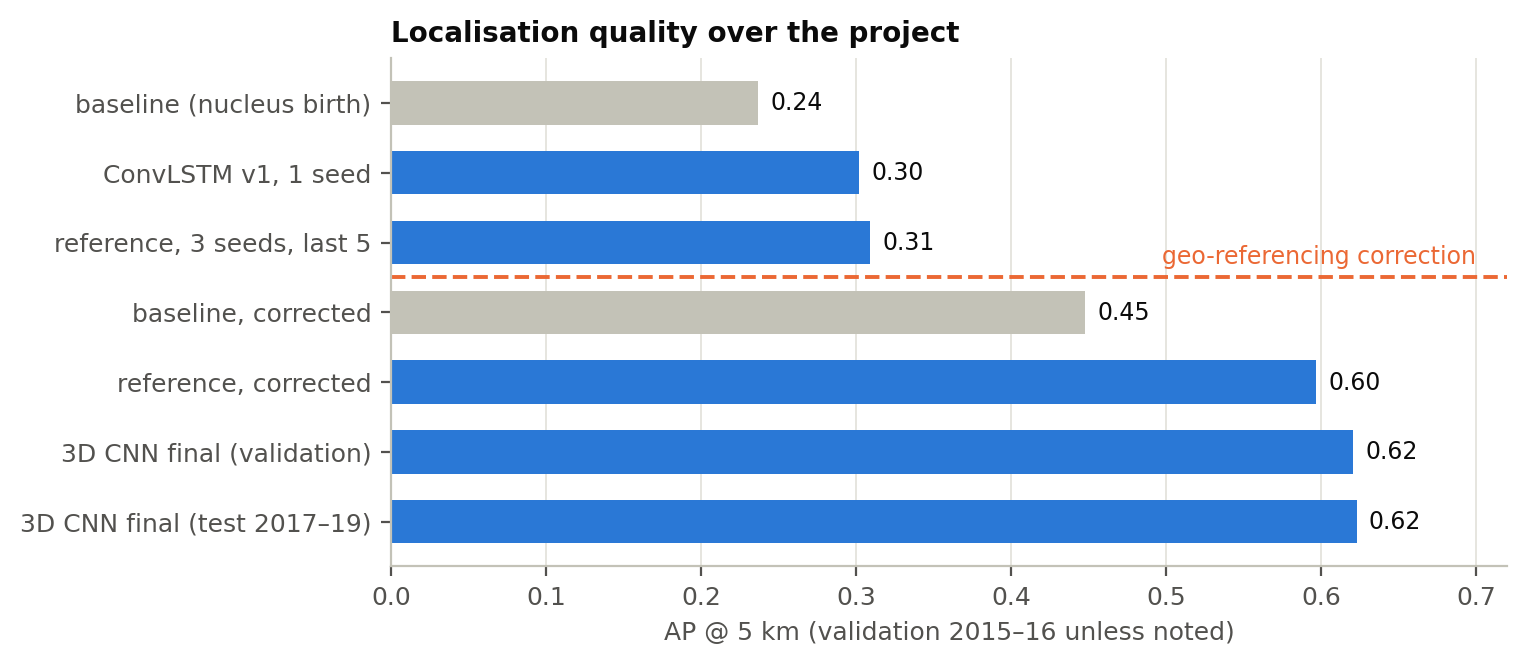
\includegraphics[width=\linewidth]{presentation/ap_progression.png}
    \column{0.45\textwidth}
    \footnotesize
    \begin{tabular}{@{}>{\raggedright\arraybackslash}p{0.40\linewidth}>{\raggedright\arraybackslash}p{0.52\linewidth}@{}}
      \toprule
      \textbf{Question} & \textbf{Answer} \\
      \midrule
      Recurrence needed? & No: 3D CNN $\geq$ ConvLSTM \\
      Bigger model? & No: 16 ch $\geq$ 32, 1 layer $\approx$ 2 \\
      FRP intensity? & Little: presence only $-0.01$ \\
      6\,h history? & Small gain ($+0.02$) \\
      Clustering as input? & No gain \\
      Hard negatives? & $\times 2$: $+0.015$ \\
      15-min steps? & No gain at $4\times$ cost \\
      \bottomrule
    \end{tabular}\\[4pt]
    \raggedright All variants within $\pm 0.03$ AP $\Rightarrow$ \textbf{limited by labels and data, not by architecture.}
  \end{columns}
\end{frame}

\begin{frame}{Test results 2017--2019 (evaluated once)}
  \begin{columns}[T]
    \column{0.6\textwidth}
    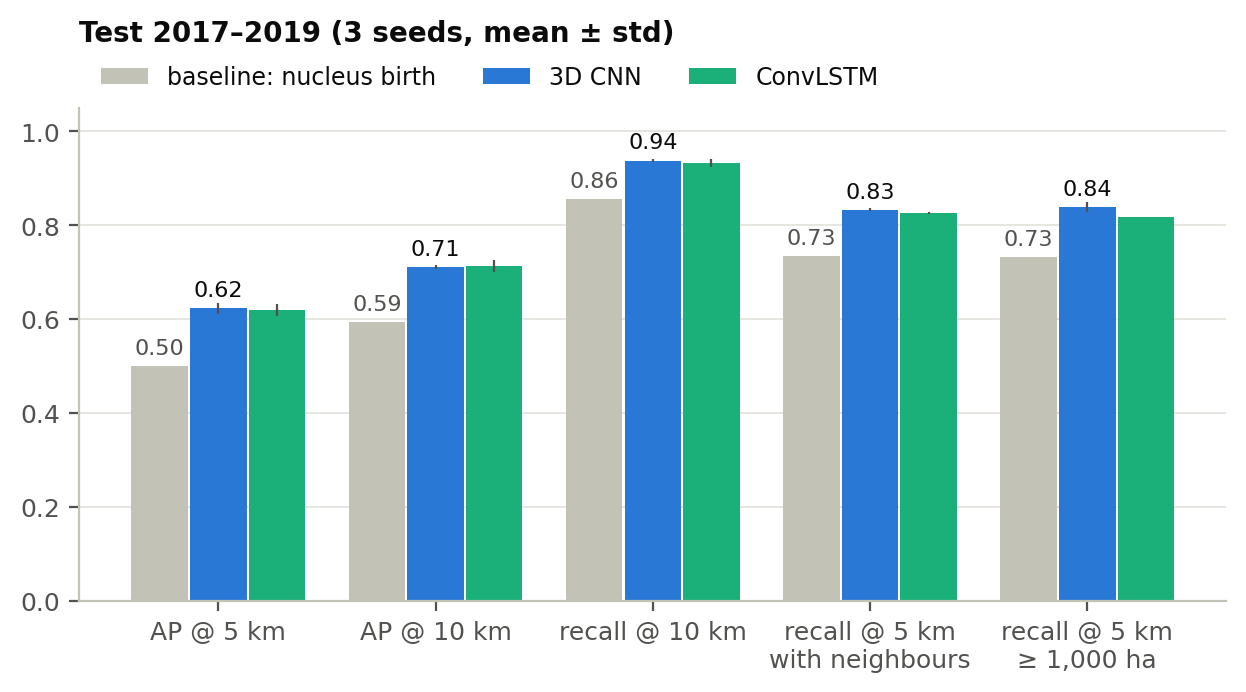
\includegraphics[width=\linewidth]{presentation/test_summary.png}
    \column{0.4\textwidth}
    \small
    \begin{itemize}
      \item +0.12 AP at both radii; fewer false alarms (0.10 vs.\ 0.15 per day)
      \item Validation numbers replicate on test (0.635 / 0.704 vs.\ 0.623 / 0.711)
      \item 3D CNN $\equiv$ ConvLSTM
      \item Largest gains for fires with neighbours and large fires
      \item Median error $\approx 2.0$\,km for both model and baseline: the gain is in \emph{finding and ranking}, not sub-pixel precision
    \end{itemize}
  \end{columns}
\end{frame}

\begin{frame}{Where it wins and where it fails}
  \begin{columns}[T]
    \column{0.58\textwidth}
    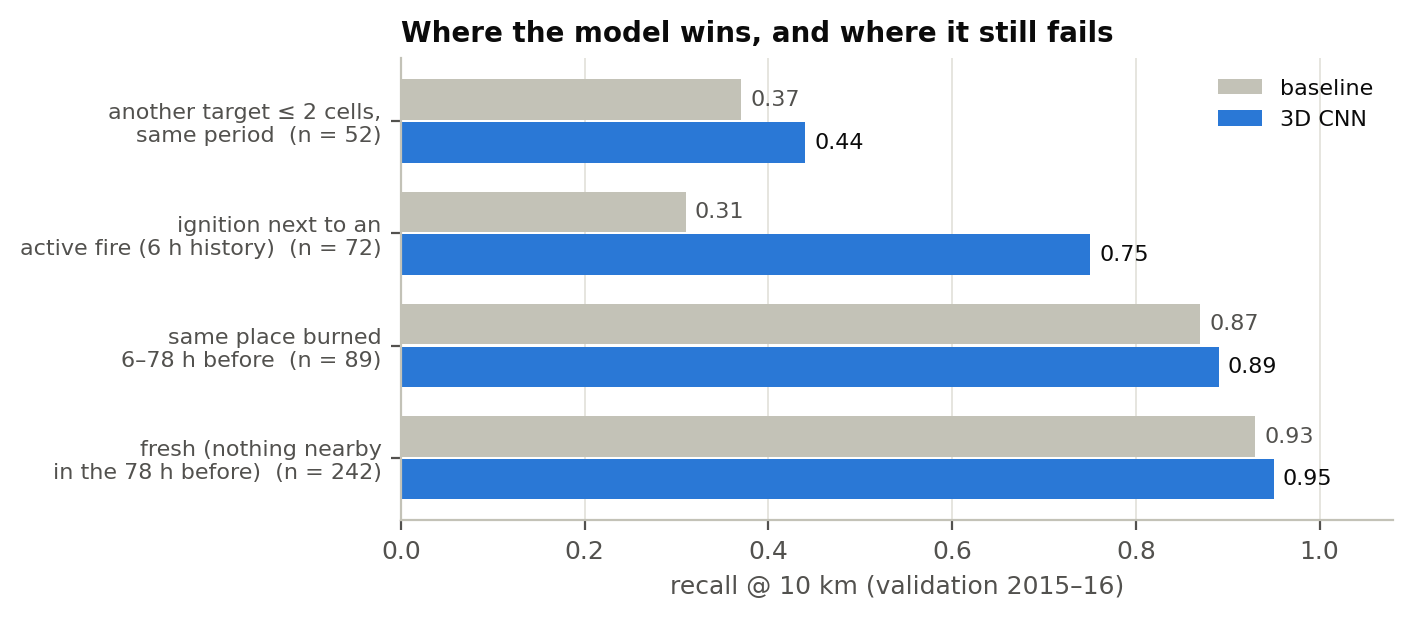
\includegraphics[width=\linewidth]{presentation/recall_by_context.png}
    \column{0.42\textwidth}
    \small
    \begin{itemize}
      \item \textbf{Win}: ignitions next to active fires (0.31 $\rightarrow$ 0.75)
      \item \textbf{Fail}: two ignitions $\leq 2$ cells apart in one period ($\approx$70\,\% of misses); typically $\sim$1.7\,h apart $\Rightarrow$ a space--\emph{time} output could separate them
      \item 58\,\% of ``false alarms'' sit on real fires (< 10\,ha, or started 1--72\,h before)
      \item Localisation floor $\approx 1.6$\,km (nearest detected pixel); model 1.9--2.0\,km
    \end{itemize}
  \end{columns}
\end{frame}

% =============================================================================
\section{Discussion}
% =============================================================================

\begin{frame}{Open points for discussion}
  \small
  \begin{columns}[T]
    \column{0.33\textwidth}
    \begin{block}{Decisions to confirm}
      \footnotesize
      \begin{itemize}
        \item Heatmap framing, $\geq 50$\,ha, ``seen'' fires only
        \item Early detection vs.\ post-fire reconstruction
        \item AP@5/10\,km as main metrics
        \item Geo-offset: own section? exact EUMETSAT date?
      \end{itemize}
    \end{block}
    \column{0.33\textwidth}
    \begin{block}{Data requests}
      \footnotesize
      \begin{itemize}
        \item SEVIRI FRP 2020--2024 (LSA SAF)
        \item SEVIRI cloud mask
        \item ICNF rekindle flag, burned-area perimeters
        \item ICNF ignition-point accuracy
        \item Full reference of ``Xu et al.\ 2025''
      \end{itemize}
    \end{block}
    \column{0.33\textwidth}
    \begin{block}{Next steps --- priority?}
      \footnotesize
      \begin{itemize}
        \item Space--time ignition output
        \item Covariates (wind, DEM, FWI) --- obj.\ iv
        \item Model 2: CNN + temporal attention (U-TAE)
        \item Explainability --- obj.\ v
        \item DEM parallax test; leave-years-out CV
      \end{itemize}
    \end{block}
  \end{columns}
  \vspace{4pt}
  \begin{alertblock}{Caveats}
    \footnotesize
    Results conditional on SEVIRI seeing the fire (19\,\% of $\geq 50$\,ha unseen) $\cdot$ ICNF positions uncertain $\cdot$
    test dominated by 2017 $\cdot$ improved decoder/ensemble not pre-registered $\cdot$ loss ablation only on uncorrected data $\cdot$ no cloud mask
  \end{alertblock}
\end{frame}

\begin{frame}[plain]
  \vfill
  \centering
  {\Huge\bfseries Discussion}\\[1em]
  \footnotesize
  \textit{Ignition Heatmaps from SEVIRI Fire Radiative Power}
  \vfill
\end{frame}

% =============================================================================
\appendix
\begin{frame}[standout]Appendix\end{frame}
% =============================================================================

\begin{frame}{A1 --- Status against the proposal objectives}
  \small
  \begin{tabular}{p{0.38\textwidth}p{0.13\textwidth}p{0.39\textwidth}}
    \toprule
    \textbf{Objective} & \textbf{Status} & \textbf{Detail} \\
    \midrule
    (i) Dataset: FRP + environment & partial & FRP part done; covariates not yet \\
    (ii) Design / evaluate architectures & partial & ConvLSTM + 3D CNN on test; Transformer open \\
    (iii) Compare modelling strategies & largely done & raw vs.\ clustered, recurrent vs.\ conv., time steps, losses \\
    (iv) Environmental variables & \textcolor{ember}{open} & needs covariates \\
    (v) Robustness, accuracy, interpretability & partial & subgroups and years done; XAI open \\
    Extension to Europe & \textcolor{ember}{not started} & optional \\
    \bottomrule
  \end{tabular}
\end{frame}

\begin{frame}{A2 --- Ablations on the corrected data}
  \centering
  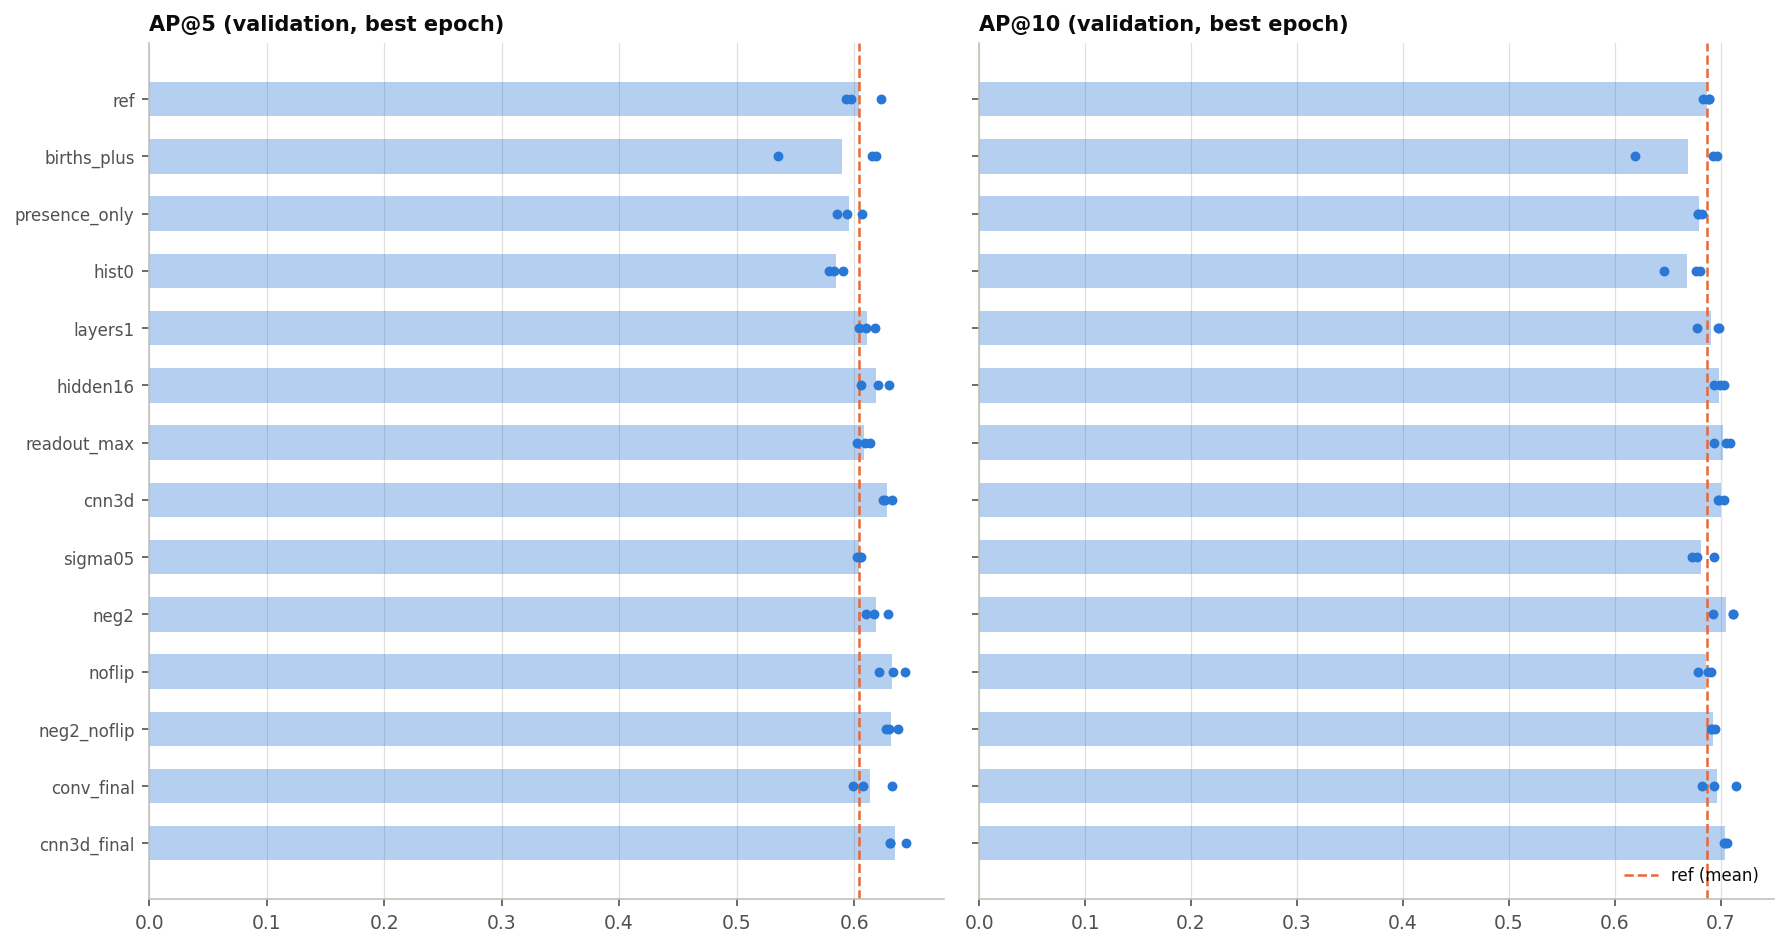
\includegraphics[height=0.7\textheight]{ablations_georef/summary.png}\\
  \src{Validation 2015--16, best epoch; dots = seeds, dashed line = reference mean.}
\end{frame}

\begin{frame}{A3 --- Precision--recall curves on test}
  \centering
  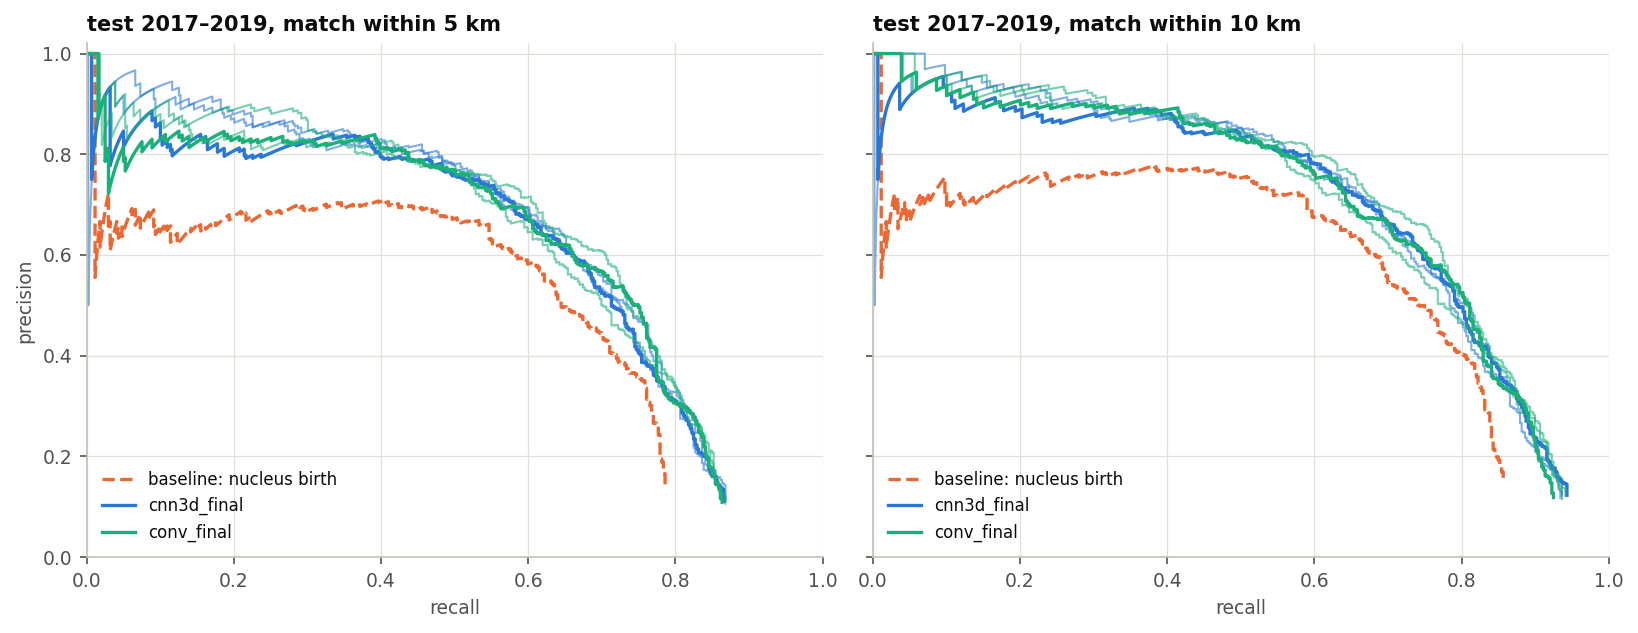
\includegraphics[width=0.85\linewidth]{final/test_pr.png}\\[4pt]
  \small
  \begin{tabular}{lccc}
    \toprule
    AP@5 / 10\,km & 2017 & 2018 & 2019 \\
    \midrule
    Baseline & 0.45 / 0.55 & 0.71 / 0.77 & 0.68 / 0.75 \\
    3D CNN & 0.58 / 0.68 & 0.85 / 0.85 & 0.73 / 0.80 \\
    ConvLSTM & 0.59 / 0.69 & 0.86 / 0.86 & 0.68 / 0.77 \\
    \bottomrule
  \end{tabular}
\end{frame}

\begin{frame}{A4 --- ConvLSTM architecture}
  \centering
  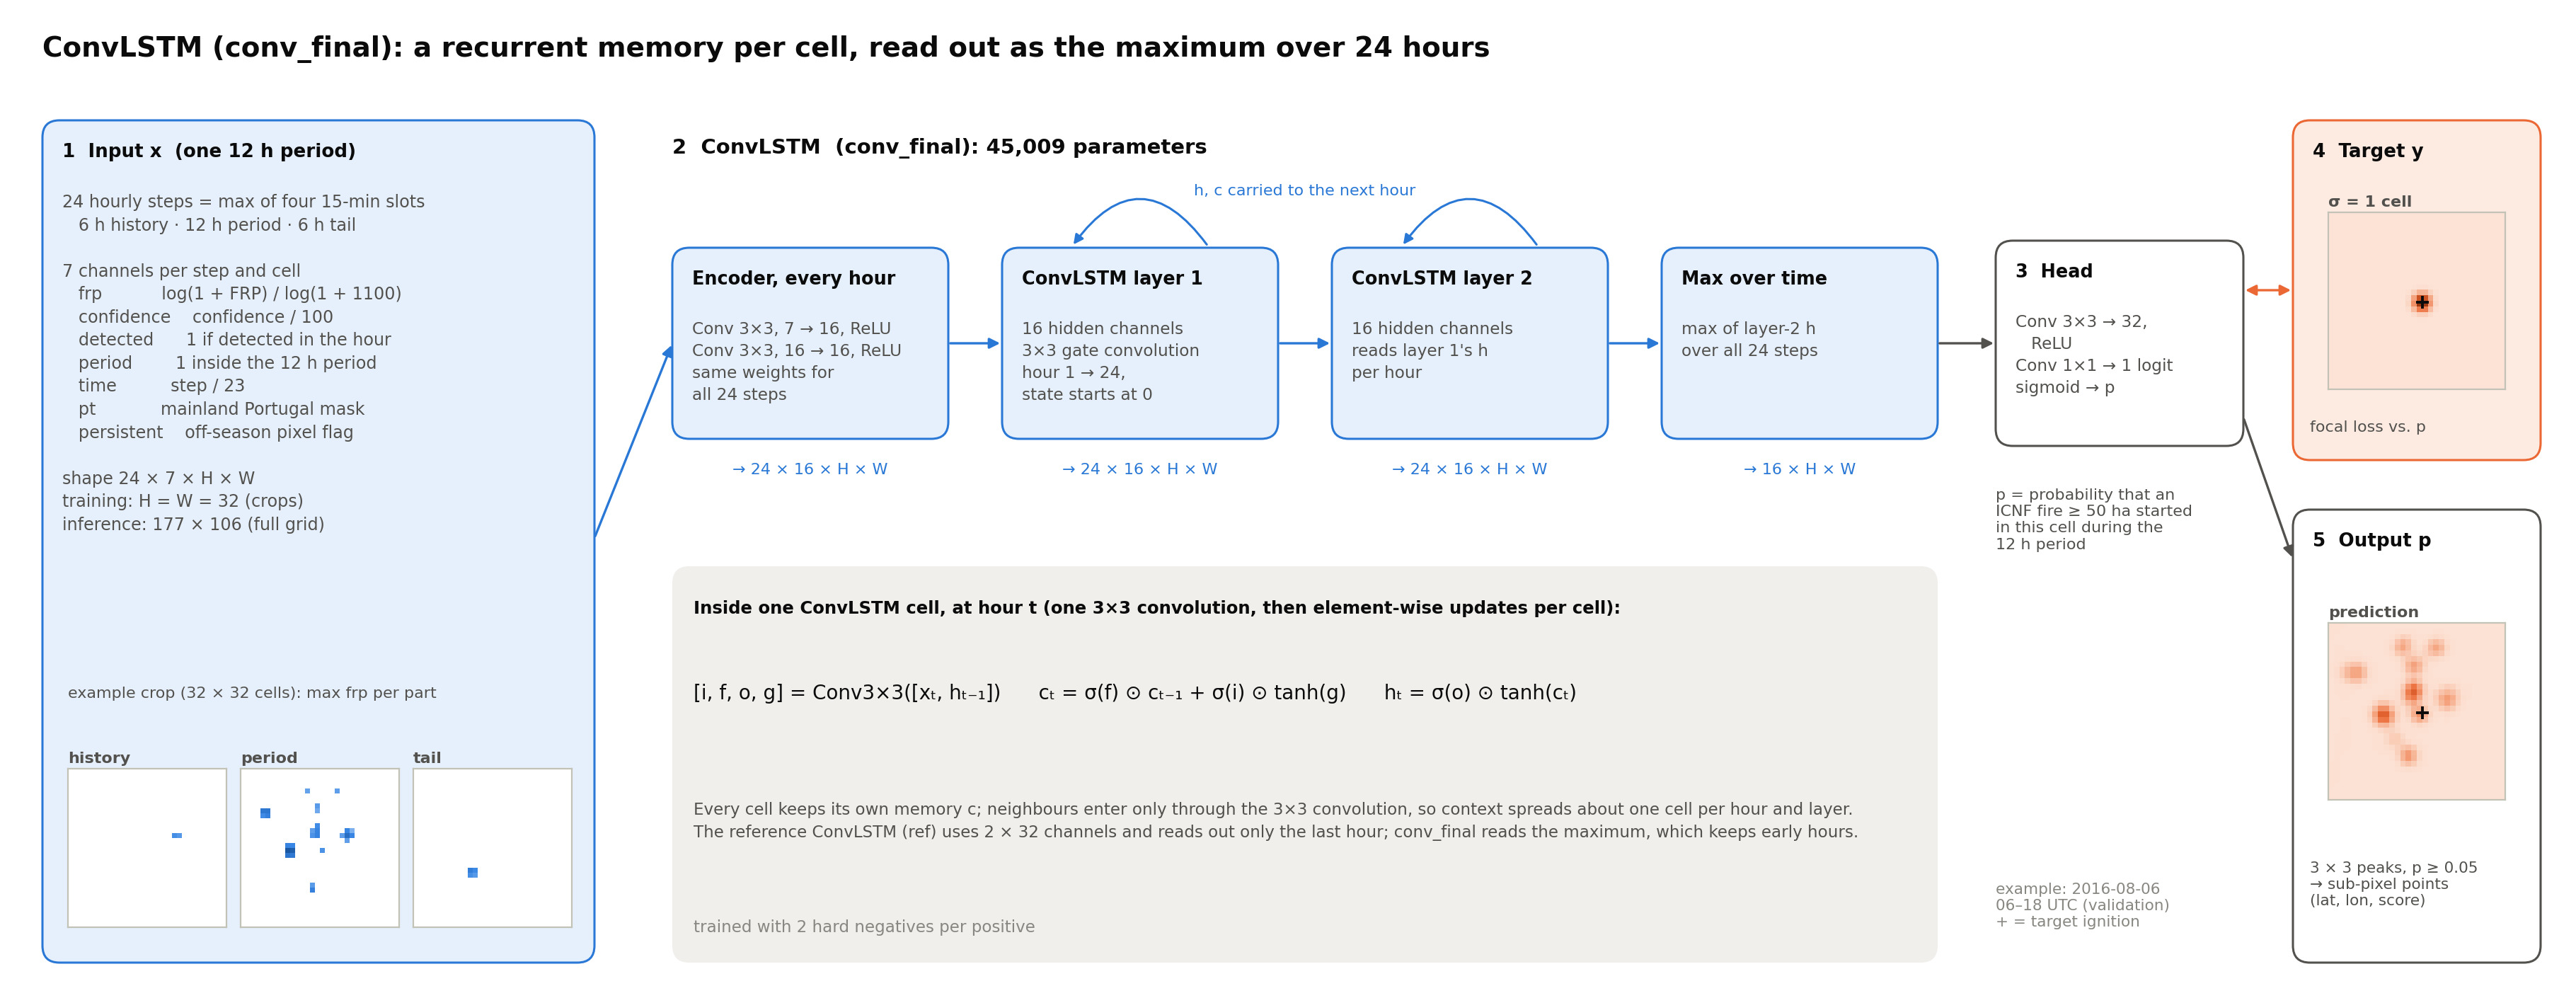
\includegraphics[width=\linewidth]{model/model_convlstm.png}
\end{frame}

\begin{frame}{A5 --- Geo-referencing correction for one fire}
  \begin{columns}[T]
    \column{0.4\textwidth}
    \centering
    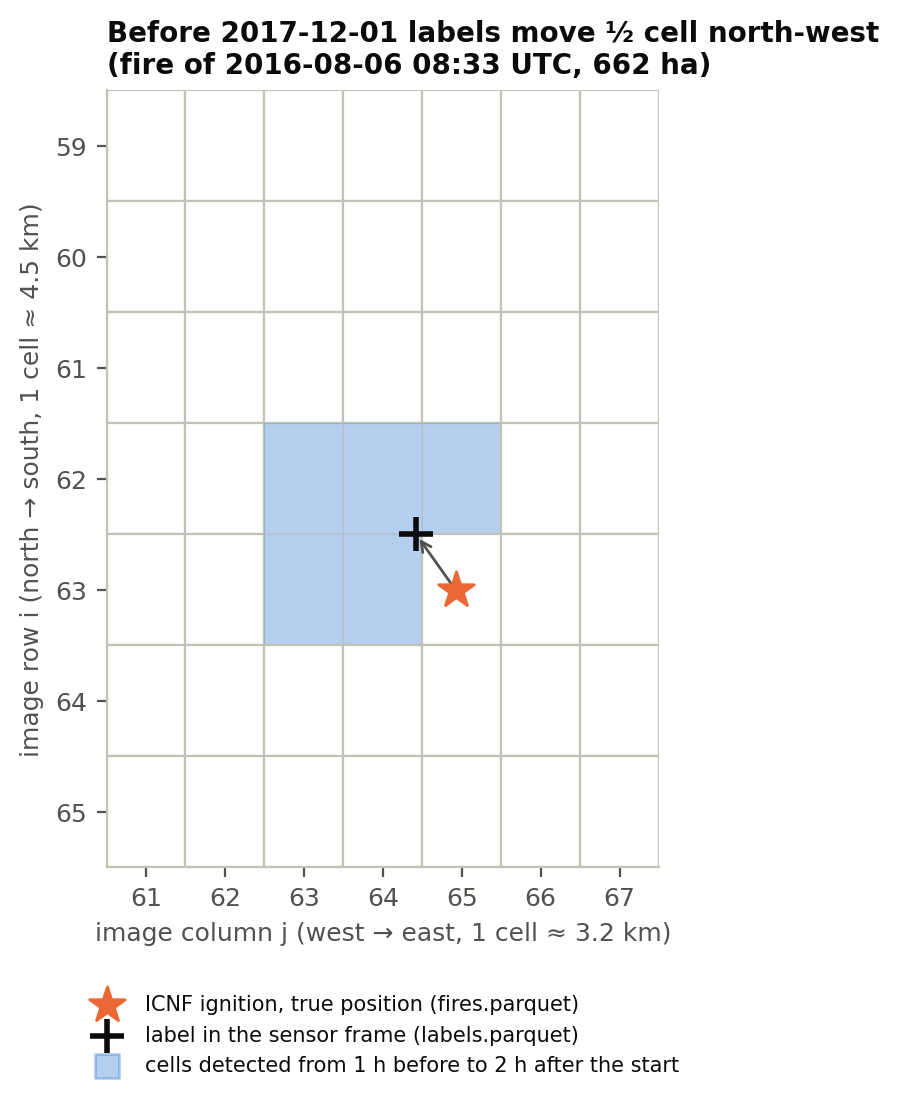
\includegraphics[height=0.78\textheight]{pipeline/georef_frames.png}
    \column{0.6\textwidth}
    \small
    \begin{itemize}
      \item Detections stay on their exact native pixels
      \item Labels before 2017-12-01 are moved half a cell north-west into the sensor frame
      \item Predictions are moved back before scoring against ICNF
      \item Remaining $\approx 0.2$ cell southward offset in both periods, larger in mountain districts\\
            $\Rightarrow$ hypothesis: \textbf{terrain parallax} (satellite views from the south at $\approx 47^\circ$); testable with a DEM
    \end{itemize}
  \end{columns}
\end{frame}

\begin{frame}{A6 --- Positioning in the literature}
  \small
  \begin{columns}[T]
    \column{0.5\textwidth}
    \begin{block}{Four strands; none learns ignition location from geostationary FRP}
      \footnotesize
      \begin{itemize}
        \item Geostationary detection/FRP (Wooster 2015; Koltunov 2016)
        \item Rule-based events and ignitions (Benali 2016; Andela 2019; Oom 2016; Chen 2022)
        \item DL on fire time series, mostly forward (Huot 2022; Gerard 2023); Pinto 2020 dates burning
        \item Generic: ConvLSTM, U-TAE, CenterNet / CornerNet / DARK
      \end{itemize}
    \end{block}
    \column{0.5\textwidth}
    \begin{block}{Closest connections}
      \footnotesize
      \begin{itemize}
        \item \textbf{Benali 2016}: same country and ICNF; rule-based; $\sim$2\,km / 12\,h
        \item \textbf{Pinto 2020 (BA-Net)}: CNN + LSTM ablation, erase augmentation, per-pixel dating
        \item \textbf{OpenSTL (Tan 2023)}: recurrence-free $\approx$ ConvLSTM
        \item \textbf{Oom 2016 / FIRED}: cluster thresholds drive results
        \item \textbf{Paugam et al.\ 2026}: MTG-FCI tracking (successor sensor)
      \end{itemize}
    \end{block}
  \end{columns}
\end{frame}

\begin{frame}{A7 --- Key references}
  \scriptsize
  \begin{itemize}
    \item Andela, N., et al.\ (2019). The Global Fire Atlas of individual fire size, duration, speed and direction. \textit{Earth Syst.\ Sci.\ Data}, 11.
    \item Benali, A., et al.\ (2016). Determining fire dates and locating ignition points with satellite data. \textit{Remote Sensing}, 8(4), 326.
    \item Chen, Y., et al.\ (2022). California wildfire spread derived using VIIRS satellite observations and an object-based tracking system. \textit{Scientific Data}, 9.
    \item Garnot, V.\ S.\ F., \& Landrieu, L.\ (2021). Panoptic segmentation of satellite image time series with convolutional temporal attention networks. \textit{ICCV}.
    \item Law, H., \& Deng, J.\ (2018). CornerNet: Detecting objects as paired keypoints. \textit{ECCV}.
    \item Lin, T.-Y., et al.\ (2017). Focal loss for dense object detection. \textit{ICCV}.
    \item Oom, D., et al.\ (2016). Biome-specific sensitivity of fire size distributions to the time-gap parameter. \textit{Remote Sensing}, 8, 663.
    \item Pinto, M.\ M., et al.\ (2020). A deep learning approach for mapping and dating burned areas using temporal sequences of satellite images. \textit{ISPRS J.\ Photogramm.}, 160.
    \item Shi, X., et al.\ (2015). Convolutional LSTM network: A machine learning approach for precipitation nowcasting. \textit{NeurIPS}.
    \item Tan, C., et al.\ (2023). OpenSTL: A comprehensive benchmark of spatio-temporal predictive learning. \textit{NeurIPS Datasets \& Benchmarks}.
    \item Wooster, M.\ J., et al.\ (2015). LSA SAF Meteosat FRP products --- Part 1. \textit{Atmos.\ Chem.\ Phys.}, 15.
    \item Zhou, X., Wang, D., \& Krähenbühl, P.\ (2019). Objects as points. arXiv:1904.07850.
  \end{itemize}
\end{frame}

\end{document}
